

Given a Lie group, we have seen how we can construct a Lie algebra as the space of left-invariant vector fields or, equivalently, tangent vectors at the identity. We will later explore the opposite direction, i.e.\ given a Lie algebra, we will see how to construct a Lie group whose associated Lie algebra is the one we started from. 

However, here we will consider a question that is independent of where a Lie algebra comes from, namely that of the classification of Lie algebras.

\subsection{Lie algebras}

While it is possible to classify Lie algebras more generally, we will only consider the classification of finite-dimensional complex Lie algebras, i.e.\ Lie algebras $(L,[-,-])$ where $L$ is a finite-dimensional $\C$-vector space. 

\be
Of course, any complex Lie group $G$ (where $G$ is a complex manifold) gives rise to a complex Lie algebra.
\ee

If $A,B$ are Lie subalgebras of a Lie algebra $(L,[-,-])$ over $K$, then
\bse
[A,B] := \lspan_K\bigl(\{[x,y]\in L \mid x\in A \text{ and } y\in B\}\bigr)
\ese
is again a Lie subalgebra of $L$.

\bd
A Lie algebra $L$ is said to be \emph{abelian} if
\bse
\forall \, x,y \in L : \ [x,y] = 0.
\ese
Equivalently, $[L,L]=0$, where $0$ denotes the trivial Lie algebra $\{0\}$.
\ed
Abelian Lie algebras are highly non-interesting as Lie algebras: since the bracket is identically zero, it may as well not be there. Even from the classification point of view, the vanishing of the bracket implies that, given any two abelian Lie algebras, every linear isomorphism between their underlying vector spaces is automatically a Lie algebra isomorphism. Therefore, for each $n\in \N$, there is (up to isomorphism) only one abelian $n$-dimensional Lie algebra.
\bd
An \emph{ideal}\index{ideal} $I$ of a Lie algebra $L$ is a Lie subalgebra such that $[I,L]\se I$, i.e.\
\bse
\forall \, x\in I : \forall \, y\in L : \ [x,y]\in I.
\ese
The ideals $0$ and $L$ are called the \emph{trivial ideals} of $L$.
\ed

\bd
A Lie algebra $L$ is said to be 
\begin{itemize}
\item \emph{simple} if it is non-abelian and it contains no non-trivial ideals;
\item \emph{semi-simple} if it contains no non-trivial abelian ideals.
\end{itemize}
\ed

\br
Note that any simple Lie algebra is also semi-simple. The requirement that a simple Lie algebra be non-abelian is due to the $1$-dimensional abelian Lie algebra, which would otherwise be the only simple Lie algebra which is not semi-simple.
\er

\bd
Let $L$ be a Lie algebra. The Lie subalgebra
\bse
L':=[L,L]
\ese
is called the \emph{derived subalgebra}\index{derived subalgebra} of $L$.
\ed

We can form a sequence of Lie subalgebras
\bse
L \supseteq L' \supseteq L'' \supseteq \cdots \supseteq L^{(n)} \supseteq \cdots
\ese
called the \emph{derived series} of $L$.

\bd
A Lie algebra $L$ is \emph{solvable} if there exists $k\in \N$ such that $L^{(k)}=0$.
\ed

Recall that the direct sum of vector spaces $V\oplus W$ has $V\times W$ as its underlying set and operations defined componentwise.

\bd
Let $L_1$ and $L_2$ be Lie algebras. The \emph{direct sum} $L_1\oplus_\mathrm{Lie}L_2$ has $L_1\oplus L_2$ as its underlying vector space and Lie bracket defined as
\bse
[x_1+x_2,y_1+y_2]_{L_1\oplus_\mathrm{Lie}L_2} := [x_1,y_1]_{L_1} + [x_2,y_2]_{L_2}
\ese
for all $x_1,y_1\in L_1$ and $x_2,y_2\in L_2$. Alternatively, by identifying $L_1$ and $L_2$ with the subspaces $L_1\oplus 0$ and $0\oplus L_2$ of $L_1\oplus L_2$ respectively, we require
\bse
[L_1,L_2]_{L_1\oplus_\mathrm{Lie}L_2} = 0.
\ese
In the following, we will drop the ``Lie'' subscript and understand $\oplus$ to mean $\oplus_\mathrm{Lie}$ whenever the summands are Lie algebras.
\ed
There is a weaker notion than the direct sum, defined only for Lie algebras.
\bd
Let $R$ and $L$ be Lie algebras. The \emph{semi-direct sum} $R\oplus_s L$ has $R\oplus L$ as its underlying vector space and Lie bracket satisfying
\bse
[R,L]_{R \oplus_s L} \se R,
\ese
i.e.\ $R$ is an ideal of $R\oplus_s L$.
\ed

We are now ready to state Levi's decomposition theorem.

\begin{theorem}[Levi]
Any finite-dimensional complex Lie algebra $L$ can be decomposed as
\bse
L = R \oplus_s (L_1 \oplus\cdots  \oplus L_n)
\ese
where $R$ is a solvable Lie algebra and $L_1,\ldots,L_n$ are simple Lie algebras.
\end{theorem}

As of today, no general classification of solvable Lie algebras is known, except for some special cases (e.g. in low dimensions). In contrast, the finite dimensional, simple, complex Lie algebras have been classified completely. % From now on, we will assume our Lie algebras to be complex unless otherwise stated.

\bp
A Lie algebra is semi-simple if, and only if, it can be expressed as a direct sum of simple Lie algebras.
\ep

Hence, the simple Lie algebras are the basic building blocks from which one can build any semi-simple Lie algebra. Then, by Levi's theorem, the classification of simple Lie algebras easily extends to a classification of all semi-simple Lie algebras.

\subsection{The adjoint map and the Killing form}

\bd
Let $L$ be a Lie algebra over $k$ and let $x\in L$. The \emph{adjoint map}\index{adjoint map} with respect to $x$ is the $K$-linear map
\bi{rrCl}
\ad_x\cl & L & \xrightarrow{\sim} & L\\
& y & \mapsto & \ad_x(y):=[x,y].
\ei
\ed

The linearity of $\ad_x$ follows from the linearity of the bracket in the second argument, while the linearity in the first argument of the bracket implies that the map
\bi{rrCl}
\ad\cl & L & \xrightarrow{\sim} & \End(L)\\
& x & \mapsto & \ad(x):=\ad_x.
\ei
itself is also linear. In fact, more is true. Recall that $\End(L)$ is a Lie algebra with bracket
\bse
[\phi,\psi]:=\phi\circ\psi-\psi\circ\phi.
\ese
Then, we have the following.
\bp
The map $\ad\cl L \xrightarrow{\sim}  \End(L)$ is a Lie algebra homomorphism.
\ep
\bq
It remains to check that $\ad$ preserves the brackets. Let $x,y,z\in L$. Then
\bi{rCl"s}
\ad_{[x,y]}(z) & := & [[x,y],z] & (definition of $\ad$)\\
& = & -[[y,z],x]-[[z,x],y] & (Jacobi's identity)\\
& = & [x,[y,z]]-[y,[x,z]] & (anti-symmetry)\\
& = & \ad_x(\ad_y(z))-\ad_y(\ad_x(z)) \\
& = & (\ad_x\circ \ad_y-\ad_y\circ \ad_x)(z)\\
& = & [\ad_x, \ad_y](z).
\ei
Hence, we have $\ad([x,y])=[\ad(x),\ad(y)]$.
\eq

\bd
Let $L$ be a Lie algebra over $K$. The \emph{Killing form}\index{Killing form} on $L$ is the $K$-bilinear map
\bi{rrCl}
\kappa \cl & L\times L & \to & K \\
& (x,y) & \mapsto & \kappa(x,y):= \tr(\ad_x\circ\ad_y),
\ei
where $\tr$ is the usual trace on the vector space $\End(L)$.
\ed
Note that the Killing form is not a ``form'' in the sense that we defined previously. In fact, since $L$ is finite-dimensional, the trace is cyclic and thus $\kappa$ is symmetric, i.e.\
\bse
\forall \, x,y\in L : \ \kappa(x,y) = \kappa(y,x).
\ese
An important property of $\kappa$ is its associativity with respect to the bracket.
\bp
Let $L$ be a Lie algebra. For any $x,y,z\in L$, we have
\bse
\kappa([x,y],z)=\kappa(x,[y,z]).
\ese
\ep
\bq
This follows easily from the fact that $\ad$ is a homomorphism.
\bi{rCl}
\kappa([x,y],z) & := & \tr(\ad_{[x,y]}\circ\ad_z)\\
& = & \tr([\ad_x,\ad_y]\circ\ad_z)\\
& = & \tr((\ad_x \circ \ad_y-\ad_y\circ\ad_x)\circ\ad_z)\\
& = & \tr(\ad_x \circ \ad_y\circ\ad_z)-\tr(\ad_y\circ\ad_x\circ\ad_z)\\
& = & \tr(\ad_x \circ \ad_y\circ\ad_z)-\tr(\ad_x\circ\ad_z\circ\ad_y)\\
& = & \tr(\ad_x \circ\, (\ad_y\circ\ad_z-\ad_z\circ\ad_y))\\
& = & \tr(\ad_x \circ\, [\ad_y,\ad_z])\\
& = & \tr(\ad_x \circ \ad_{[y,z]})\\
& =: & \kappa(x,[y,z]),
\ei
where we used the cyclicity of the trace.
\eq

We can use $\kappa$ to give a further equivalent characterisation of semi-simplicity.

\bp[Cartan's criterion]\index{Cartan's criterion}
A Lie algebra $L$ is semi-simple if, and only if, the Killing form $\kappa$ is non-degenerate, i.e.\
\bse
(\forall \, y \in L : \kappa(x,y)=0) \Rightarrow x = 0.
\ese
\ep
Hence, if $L$ is semi-simple, then $\kappa$ is a pseudo inner product on $L$. Recall the following definition from linear algebra.

\bd
A linear map $\phi\cl V\xrightarrow{\sim}V$ is said to be \emph{symmetric} with respect to the pseudo inner product $B(-,-)$ on $V$ if
\bse
\forall \, v,w\in V : \ B(\phi(v),w)=B(v,\phi(w)).
\ese
If, instead, we have
\bse
\forall \, v,w\in V : \ B(\phi(v),w)=-B(v,\phi(w)),
\ese
then $\phi$ is said to be \emph{anti-symmetric} with respect to $B$.
\ed
The associativity property of $\kappa$ with respect to the bracket can be restated by saying that, for any $z\in L$, the linear map $\ad_z$ is anti-symmetric with respect to $\kappa$, i.e.\
\bse
\forall \, x,y\in L : \ \kappa(\ad_z(x),y) = - \kappa(x,\ad_z(y)). 
\ese

In order to do computations, it is useful to introduce a basis $\{E_i\}$ on $L$.
\bd
Let $L$ be a Lie algebra over $K$ and let $\{E_i\}$ be a basis. Then, we have
\bse
[E_i,E_j] = C^{k}_{\phantom{k}ij}E_k
\ese
for some $C^{k}_{\phantom{k}ij}\in K$. The numbers $C^{k}_{\phantom{k}ij}$ are called the \emph{structure constants}\index{structure constants} of $L$ with respect to the basis $\{E_i\}$.
\ed
In terms of the structure constants, the anti-symmetry of the Lie bracket reads
\bse
 C^{k}_{\phantom{k}ij} = - C^{k}_{\phantom{k}ji}
\ese
while the Jacobi identity becomes
\bse
C^{n}_{\phantom{n}im}C^{m}_{\phantom{m}jk} +  C^{n}_{\phantom{n}jm}C^{m}_{\phantom{m}ki} + C^{n}_{\phantom{n}km}C^{m}_{\phantom{m}ij} = 0.
\ese

We can now express both the adjoint maps and the Killing form in terms of components with respect to a basis.
\bp
Let $L$ be a Lie algebra and let $\{E_i\}$ be a basis. Then
\ben[label=\roman*)]
\item $(\ad_{E_i})^k_{\phantom{k}j} = C^{k}_{\phantom{k}ij}$
\item $\kappa_{ij}=C^m_{\phantom{m}ik}C^k_{\phantom{k}jm}$
\een
where $C^{k}_{\phantom{k}ij}$ are the structure constants of $L$ with respect to $\{E_i\}$.
\ep
\bq
\ben[label=\roman*)]
\item Denote by $\{\varepsilon^i\}$ the dual basis to $\{E_i\}$. Then, we have
\bi{rCl}
(\ad_{E_i})^k_{\phantom{k}j} &:=& \varepsilon^k(\ad_{E_i}(E_j)) \\
& = & \varepsilon^k ([E_i,E_j])\\
& = & \varepsilon^k (C^{m}_{\phantom{\,m}ij}E_m)\\
& = & C^{m}_{\phantom{m}ij}\varepsilon^k (E_m)\\
&=& C^{k}_{\phantom{k}ij},
\ei
since $\varepsilon^k(E_m)=\delta^k_m$.
\item Recall from linear algebra that if $V$ is finite-dimensional, for any $\phi\in\End(V)$ we have $\tr(\phi)=\Phi^k_{\phantom{k}k}$, where $\Phi$ is the matrix representing the linear map in any basis. Also, recall that the matrix representing $\phi\circ\psi$ is the product $\Phi\Psi$. Using these, we have
\bi{rCl}
\kappa_{ij} &:= & \kappa(E_i,E_j)\\
& = & \tr(\ad_{E_i}\circ\ad_{E_j})\\
& = & ( \ad_{E_i}\circ\ad_{E_j} )^k_{\phantom{k}k}\\
& = & ( \ad_{E_i})^m_{\phantom{m}k}(\ad_{E_j} )^k_{\phantom{k}m}\\
& = & C^m_{\phantom{m}ik}C^k_{\phantom{k}jm},
\ei 
where we used the same notation for the linear maps and their matrices.\qedhere
\een
\eq

\subsection{The fundamental roots and the Weyl group}

We will now focus on finite-dimensional semi-simple complex Lie algebras, whose classification hinges on the existence of a special type of subalgebra.

\bd
Let $L$ be a $d$-dimensional Lie algebra. A \emph{Cartan subalgebra}\index{Cartan subalgebra} $H$ of $L$ is a maximal Lie subalgebra of $L$ with the following property: there exists a basis $\{h_1,\ldots,h_r\}$ of $H$ which can be extended to a basis $\{h_1,\ldots,h_r,e_1,\ldots,e_{d-r}\}$ of $L$ such that $e_1,\ldots,e_{d-r}$ are eigenvectors of $\ad(h)$ for any $h\in H$, i.e.\
\bse
\forall \, h\in H : \exists \, \lambda_\alpha(h)\in \C : \ \ad(h)e_\alpha = \lambda_\alpha(h) e_\alpha,
\ese
for each $1\leq\alpha\leq d-r$.
\ed

The basis $\{h_1,\ldots,h_r,e_1,\ldots,e_{d-r}\}$ is known as a \emph{Cartan-Weyl basis}\index{Cartan-Weyl basis} of $L$.
%Of course, we would like to know when we can find such a subalgebra.

\begin{theorem}
Let $L$ be a finite-dimensional semi-simple complex Lie algebra. Then
\ben[label=\roman*)]
\item $L$ possesses a Cartan subalgebra;
\item all Cartan subalgebras of $L$ have the same dimension, called the \emph{rank} of $L$;
\item any of Cartan subalgebra of $L$ is abelian.
\een
\end{theorem}

Note that we can think of the $\lambda_\alpha$ appearing above as a map $\lambda_\alpha\cl H \to \C$. Moreover, for any $z\in \C$ and $h,h'\in H$, we have
\bi{rCl}
\lambda_\alpha(zh+h') e_\alpha  & = & \ad(zh+h') e_\alpha\\
& = & [zh+h',e_\alpha] \\
& = & z[h,e_\alpha] + [h',e_\alpha] \\
& = & z\lambda_\alpha(h)e_\alpha +\lambda_\alpha(h')e_\alpha\\
& = & (z\lambda_\alpha(h)+\lambda_\alpha(h')) e_\alpha,
\ei
Hence $\lambda_\alpha$ is a $\C$-linear map $\lambda_\alpha\cl H \xrightarrow{\sim}\C$, and thus $\lambda_\alpha\in H^*$.

\bd
The maps $\lambda_1,\ldots,\lambda_{d-r}\in H^*$ are called the \emph{roots}\index{root} of $L$. The collection
\bse
\Phi := \{\lambda_\alpha \mid 1\leq \alpha \leq d-r\} \se H^*
\ese
is called the \emph{root set} of $L$.
\ed

One can show that if $\lambda_\alpha$ were the zero map, then we would have $e_\alpha\in H$. Thus, we must have $0\notin \Phi$. Note that a consequence of the anti-symmetry of each $\ad(h)$ with respect to the Killing form $\kappa$ is that
\bse
\lambda \in \Phi\ \Rightarrow\ -\lambda\in \Phi.
\ese
Hence $\Phi$ is not a linearly independent subset of $H^*$.

\bd
A set of \emph{fundamental roots}\index{fundamental root} $\Pi:=\{\pi_1,\ldots,\pi_f\}$ is a subset $\Pi\se\Phi$ such that 
\ben[label=\alph*)]
\item $\Pi$ is a linearly independent subset of $H^*$;
\item for each $\lambda \in \Phi$, there exist $n_1,\ldots,n_f\in \N$ and $\varepsilon \in \{+1,-1\}$ such that
\bse
\lambda = \varepsilon \, \sum_{i=1}^f n_i \pi_i.
\ese
\een
\ed
We can write the last equation more concisely as $\lambda \in \lspan_{\varepsilon,\N}(\Pi)$. Observe that, for any $\lambda\in \Phi$, the coefficients of $\pi_1,\ldots,\pi_f$ in the expansion above always have the same sign. Indeed, we have $\lspan_{\varepsilon,\N}(\Pi)\neq \lspan_{\Z}(\Pi)$. 

\begin{theorem}
Let $L$ be a finite-dimensional semi-simple complex Lie algebra. Then
\ben[label=\roman*)]
\item a set $\Pi\se\Phi$ of fundamental roots always exists;
\item we have $\lspan_\C(\Pi) = H^*$, that is, $\Pi$ is a basis of $H^*$.
\een
\end{theorem}
\bc
We have $|\Pi| = r$, where $r$ is the rank of $L$.
\ec
\bq
Since $\Pi$ is a basis, $|\Pi| = \dim H^* = \dim H = r$.
\eq
We would now like to use $\kappa$ to define a pseudo inner product on $H^*$. We know from linear algebra that a pseudo inner product $B(-,-)$ on a finite-dimensional vector space $V$ over $K$ induces a linear isomorphism
\bi{rrCl}
i \cl & V & \xrightarrow{\sim} & V^*\\
& v & \mapsto & i(v) := B(v,-)
\ei
which can be used to define a pseudo inner product $B^*(-,-)$ on $V^*$ as
\bi{rrCl}
B^* \cl & V^*\times V^* & \to & K\\
& (\phi,\psi) & \mapsto & B^*(\phi,\psi) := B(i^{-1}(\phi),i^{-1}(\psi)).
\ei
We would like to apply this to the restriction of $\kappa$ to the Cartan subalgebra. However, a pseudo inner product on a vector space is not necessarily a pseudo inner product on a subspace, since the non-degeneracy condition may fail when considered on a subspace.
\bp
The restriction of $\kappa$ to $H$ is a pseudo inner product on $H$.
\ep
\bq
Bilinearity and symmetry are automatically satisfied. It remains to show that $\kappa$ is non-degenerate on $H$. 
\ben[label=\roman*)]
\item Let $\{h_1,\ldots,h_r,e_{r+1},\ldots,e_{d}\}$ be a Cartan-Weyl basis of $L$ and let $\lambda_\alpha\in \Phi$. Then
\bi{rCl}
\lambda_\alpha(h_j) \kappa(h_i,e_\alpha)& = & \kappa(h_i,\lambda_\alpha(h_j)e_\alpha)\\
& = & \kappa(h_i,[h_j,e_\alpha])\\
& = & \kappa([h_i,h_j],e_\alpha)\\
& = & \kappa(0,e_\alpha)\\
& = & 0.
\ei
Since $\lambda_\alpha \neq 0$, there is some $h_j$ such that $\lambda_\alpha(h_j)\neq 0$ and hence
\bse
\kappa(h_i,e_\alpha) = 0.
\ese
By linearity, we have $\kappa(h,e_\alpha)=0$ for any $h\in H$ and any $e_\alpha$.
\item Let $h\in H\se L$. Since $\kappa$ is non-degenerate on $L$, we have
\bse
\bigl(\forall \, x\in L : \kappa(h,x) = 0 \bigr) \Rightarrow h =0.
\ese
Expand $x\in L$ in the Cartan-Weyl basis as
\bse
x = h' + e  
\ese
where $h':=x^ih_i$ and $e:=x^\alpha e_\alpha$. Then, we have
\bse
\kappa(h,x) = \kappa(h,h') + x^\alpha\kappa(h,e_\alpha) = \kappa(h,h').
\ese
Thus, the non-degeneracy condition reads
\bse
\bigl(\forall \, h'\in H : \kappa(h,h') = 0 \bigr) \Rightarrow h =0,
\ese
which is what we wanted. \qedhere
\een
\eq

We can now define
\bi{rrCl}
\kappa^*\cl & H^* \times H^* & \to & \C\\
& (\mu,\nu)&\mapsto & \kappa^*(\mu,\nu):=\kappa(i^{-1}(\mu),i^{-1}(\nu)),
\ei
where $i\cl H \xrightarrow{\sim} H^*$ is the linear isomorphism induced by $\kappa$. 

\br
If $\{h_i\}$ is a basis of $H$, the components of $\kappa^*$ with respect to the dual basis satisfy 
\bse
(\kappa^*)^{ij}\kappa_{jk}=\delta^i_k.
\ese
Hence, we can write
\bse
\kappa^*(\mu,\nu)=(\kappa^*)^{ij}\mu_i\nu_j,
\ese
where $\mu_i:=\mu(h_i)$.
\er
We now turn our attention to the real subalgebra $H^*_\R:=\lspan_\R(\Pi)$. Note that  we have the following chain of inclusions
\bse
\Pi\se\Phi\se\lspan_{\varepsilon,\N}(\Pi) \se \underbrace{\lspan_\R(\Pi)}_{H_\R^*} \se \underbrace{\lspan_\C(\Pi)}_{H^*}.
\ese
The restriction of $\kappa^*$ to $H_\R^*$ leads to a surprising result.
\begin{theorem}
\ben[label=\roman*)]
\item For any $\alpha,\beta\in H_\R^*$, we have $\kappa^*(\alpha,\beta)\in \R$.
\item $\kappa^*\cl H_\R^*\times  H_\R^*\to \R$ is an inner product on $H_\R^*$.
\een
\end{theorem}
This is indeed a surprise! Upon restriction to $H_\R^*$, instead of being weakened, the non-degeneracy of $\kappa^*$ gets strengthened to positive definiteness. Now that we have a proper real inner product, we can define some familiar notions from basic linear algebra, such as lengths and angles.

\bd
Let $\alpha,\beta\in H_\R^*$. Then, we define
\ben[label=\roman*)]
\item the \emph{length} of $\alpha$ as $|\alpha|:=\sqrt{\kappa^*(\alpha,\alpha)}\,$;
\item the \emph{angle} between $\alpha$ and $\beta$ as $\ds \varphi := \cos^{-1}\biggl(\frac{\kappa^*(\alpha,\beta)}{|\alpha||\beta|}\biggr) $.
\een
\ed
We need one final ingredient for our classification result.
\bd
For any $\lambda\in \Phi\se H_\R^*$, define the linear map
\bi{rrCl}
s_\lambda \cl & H_\R^* & \xrightarrow{\sim} & H_\R^*\\
& \mu & \mapsto & s_\lambda(\mu),
\ei
where
\bse
s_\lambda(\mu):=\mu-2\frac{\kappa^*(\lambda,\mu)}{\kappa^*(\lambda,\lambda)}\,\lambda .
\ese
The map $s_\lambda$ is called a \emph{Weyl transformation} and the set
\bse
W:=\{s_\lambda \mid \lambda \in \Phi\}
\ese
is a group under composition of maps, called the \emph{Weyl group}\index{Weyl group}.
\ed

\begin{theorem}
\ben[label=\roman*)]
\item The Weyl group $W$ is generated by the fundamental roots in $\Pi$, in the sense that for some $1\leq n \leq r$, with $r=|\Pi|$,
\bse
\forall \, w \in W : \exists \, \pi_1,\ldots,\pi_n\in \Pi : \ w = s_{\pi_1} \circ s_{\pi_2} \circ\cdots  \circ s_{\pi_n} ;
\ese
\item Every root can be produced from a fundamental root by the action of $W$, i.e.\
\bse
\forall \, \lambda\in \Phi :\exists\, \pi\in \Pi :  \exists\, w\in W :\ \lambda = w(\pi);
\ese
\item The Weyl group permutes the roots, that is,
\bse
\forall \, \lambda \in \Phi : \forall \, w \in W : \ w(\lambda)\in \Phi.
\ese
\een
\end{theorem}

\subsection{Dynkin diagrams and the Cartan classification}

Consider, for any $\pi_i,\pi_j\in \Pi$, the action of the Weyl transformation
\bse
s_{\pi_i}(\pi_j) := \pi_j-2\frac{\kappa^*(\pi_i,\pi_j)}{\kappa^*(\pi_i,\pi_i)}\,\pi_i.
\ese
Since $s_{\pi_i}(\pi_j)\in\Phi$ and $\Phi\se\lspan_{\varepsilon,\N}(\Pi)$, for all $1\leq i\neq j\leq r$ we must have
\bse
-2\frac{\kappa^*(\pi_i,\pi_j)}{\kappa^*(\pi_i,\pi_i)}\in \N.
\ese
\bd
The \emph{Cartan matrix}\index{Cartan matrix} of a Lie algebra is the $r\times r$ matrix $C$ with entries
\bse
C_{ij} :=2\frac{\kappa^*(\pi_i,\pi_j)}{\kappa^*(\pi_i,\pi_i)},
\ese
where the $C_{ij}$ should not be confused with the structure constants $C^k_{\phantom{k}ij}$.
\ed
\begin{theorem}To every simple finite-dimensional complex Lie algebra there corresponds a unique Cartan matrix and vice versa (up to relabelling of the basis elements).
\end{theorem}
Of course, not every matrix can be a Cartan matrix. For instance, since $C_{ii}=2$ (no summation implied), the diagonal entries of $C$ are all equal to $2$, while the off-diagonal entries are either zero or negative. In general, $C_{ij} \neq C_{ji}$, so the Cartan matrix is not symmetric, but if $C_{ij}=0$, then necessarily $C_{ji}=0$.

We have thus reduced the problem of classifying the simple finite-dimensional complex Lie algebras to that of finding all the Cartan matrices. This can, in turn, be reduced to the problem of determining all the inequivalent Dynkin diagrams. 
\bd
Given a Cartan matrix $C$, the $ij$-th \emph{bond number} is
\bse
n_{ij}:= C_{ij} C_{ji} \qquad \text{(no summation implied)}.
\ese
\ed
Note that we have
\bi{rCl}
n_{ij} & = & 4\,\frac{\kappa^*(\pi_i,\pi_j)}{\kappa^*(\pi_i,\pi_i)}\,\frac{\kappa^*(\pi_j,\pi_i)}{\kappa^*(\pi_j,\pi_j)}\\
& = & 4\, \biggl(\frac{\kappa^*(\pi_i,\pi_j)}{|\pi_i||\pi_j|}\biggr)^2\\
& = & 4 \cos^2\varphi,
\ei
where $\varphi$ is the angle between $\pi_i$ and $\pi_j$. For $i\neq j$, the angle $\varphi$ is neither zero nor $180^\circ$, hence $0\leq \cos^2\varphi< 1$, and therefore
\bse
n_{ij}\in \{0,1,2,3\}.
\ese
Since $C_{ij}\leq 0$ for $i\neq j$, the only possibilities are
\begin{center}
%\def\arraystretch{1}
%\setlength\tabcolsep{10pt}
\begin{tabular}{ cc | c}
$C_{ij}$ & $C_{ji}$ & $n_{ij}$\\[2pt]
\hline
$\phantom{-}0$ & $\phantom{-}0\rule{0pt}{13pt}\ $ &  0 \\
$-1$ & $-1\ $ & 1\\
$-1$ & $-2\ $ & 2\\
$-1$ & $-3\ $ & 3
\end{tabular}
\end{center}
% \begin{center}
% \begin{tabular}{ r@{,}l | c}
% $(C_{ij}$ & $\,C_{ji})$ & $n_{ij}$\\[2pt]
% \hline
% $(0$ & $\,0)\rule{0pt}{13pt}\ $ &  0 \\
% $(-1$ & $\,-1) $ & 1\\
% $(-1$ & $\,-2) $ & 2\\
% $(-1$ & $\,-3) $ & 3
% \end{tabular}
% \end{center}
Note that while the Cartan matrices are not symmetric, swapping any pair of $C_{ij}$ and $C_{ji}$ gives a Cartan matrix which represents the same Lie algebra as the original matrix, with two elements from the Cartan-Weyl basis swapped. This is why we have not included $(-2,-1)$ and $(-3,-1)$ in the table above.

If $n_{ij}= 2$ or $3$, then the corresponding fundamental roots have different lengths, i.e.\ either $|\pi_i|<|\pi_j|$ or $|\pi_i|>|\pi_j|$. We also have the following result.

\bp
The roots of a simple Lie algebra have, at most, two distinct lengths.
\ep

The redundancy of the Cartan matrices highlighted above is nicely taken care of by considering Dynkin diagrams.

\bd
A \emph{Dynkin diagram}\index{Dynkin diagram} associated to a Cartan matrix is constructed as follows.
\ben
\item Draw a circle for every fundamental root in $\pi_i\in\Pi$;
\begin{center}
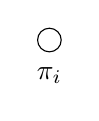
\begin{tikzpicture}
\draw[fill=white] (0,0) circle[radius=0.15];
\draw (0,-0.45) node {$\pi_i$};
\end{tikzpicture}
\end{center}
\item Draw $n_{ij}$ lines between the circles representing the roots $\pi_i$ and $\pi_j$;
\begin{center}
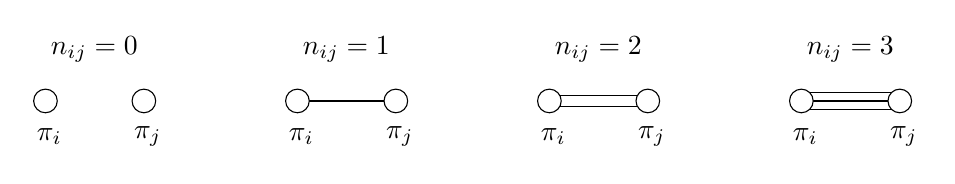
\begin{tikzpicture}
\draw (3.2,0) -- (3.2+1.25,0);
\draw (2*3.2,0.07) -- (2*3.2+1.25,0.07);
\draw (2*3.2,-0.07) -- (2*3.2+1.25,-0.07); 
\draw (3*3.2,0.11) -- (3*3.2+1.25,0.11); 
\draw (3*3.2,0) -- (3*3.2+1.25,0); 
\draw (3*3.2,-0.11) -- (3*3.2+1.25,-0.11); 
\foreach \x in {0,1,2,3} {
\draw (3.2*\x+0.62,0.65) node {$n_{ij}=\x$};
\draw (3.2*\x+0.05,-0.45) node {$\pi_i$};
\draw (3.2*\x+1.3,-0.45) node {$\pi_j$};
\draw[fill=white] (3.2*\x,0) circle[radius=0.15];
\draw[fill=white] (3.2*\x+1.25,0) circle[radius=0.15];
}
\end{tikzpicture}
\end{center}
\item If $n_{ij}=2$ or $3$, draw an arrow on the lines from the longer root to the shorter root.
\begin{center}
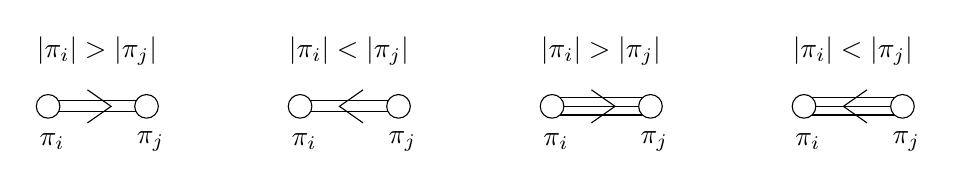
\begin{tikzpicture}
\foreach \x in {0,1} {
\draw (2*3.2*\x+0.62,0.7) node {$|\pi_i|>|\pi_j|$};
\draw (2*3.2*\x+0.65-0.15,0.21) -- (2*3.2*\x+0.65+0.15,0) -- (2*3.2*\x+0.65-0.15,-0.21);
\draw (2*3.2*\x+3.2+0.62,0.7) node {$|\pi_i|<|\pi_j|$};
\draw (2*3.2*\x+3.2+0.65+0.15,0.21) -- (2*3.2*\x+3.2+0.65-0.15,0) -- (2*3.2*\x+3.2+0.65+0.15,-0.21);
\draw (\x*3.2,0.07) -- (\x*3.2+1.25,0.07);
\draw (\x*3.2,-0.07) -- (\x*3.2+1.25,-0.07); 
}
\foreach \x in {2,3} {
\draw (\x*3.2,0.11) -- (\x*3.2+1.25,0.11); 
\draw (\x*3.2,0) -- (\x*3.2+1.25,0); 
\draw (\x*3.2,-0.11) -- (\x*3.2+1.25,-0.11); 
}
\foreach \x in {0,1,2,3} {
\draw (3.2*\x+0.05,-0.45) node {$\pi_i$};
\draw (3.2*\x+1.3,-0.45) node {$\pi_j$};
\draw[fill=white] (3.2*\x,0) circle[radius=0.15];
\draw[fill=white] (3.2*\x+1.25,0) circle[radius=0.15];
}
\end{tikzpicture}
\end{center}
\een
\ed
Dynkin diagrams completely characterise any set of fundamental roots, from which we can reconstruct the entire root set by using the Weyl transformations. The root set can then be used to produce a Cartan-Weyl basis.

We are now finally ready to state the much awaited classification theorem.
\begin{theorem}[Killing, Cartan]\index{Cartan classification}
Any simple finite-dimensional complex Lie algebra can be reconstructed from its set of fundamental roots $\Pi$, which only come in the following forms. 
\ben[label=\roman*)]
\item There are $4$ infinite families
% \bi{rCl}
% A_n & n \geq 1 & 
% \begin{tikzpicture}
% \draw (0,0) edge (2*1.25,0);
% \draw (2*1.25,0) edge[dashed] (3*1.25,0);
% \draw (3*1.25,0) edge (4*1.25,0);
% \foreach \x in {0,1,2,3,4} {
% \draw[fill=white] (1.25*\x,0) circle[radius=0.15];
% }
% \end{tikzpicture}\\
% B_n & n \geq 2 & 
% \begin{tikzpicture}
% \draw (0,0) edge (2*1.25,0);
% \draw (2*1.25,0) edge[dashed] (3*1.25,0);
% \draw (3*1.25+0.65-0.15,0.21) -- (3*1.25+0.65+0.15,0) -- (3*1.25+0.65-0.15,-0.21);
% \draw (3*1.25,0.07) -- (4*1.25,0.07);
% \draw (3*1.25,-0.07) -- (4*1.25,-0.07); 
% \foreach \x in {0,1,2,3,4} {
% \draw[fill=white] (1.25*\x,0) circle[radius=0.15];
% }
% \end{tikzpicture}\\
% C_n & n \geq 3 & 
% \begin{tikzpicture}
% \draw (0,0) edge (2*1.25,0);
% \draw (2*1.25,0) edge[dashed] (3*1.25,0);
% \draw (3*1.25+0.65+0.15,0.21) -- (3*1.25+0.65-0.15,0) -- (3*1.25+0.65+0.15,-0.21);
% \draw (3*1.25,0.07) -- (4*1.25,0.07);
% \draw (3*1.25,-0.07) -- (4*1.25,-0.07); 
% \foreach \x in {0,1,2,3,4} {
% \draw[fill=white] (1.25*\x,0) circle[radius=0.15];
% }
% \end{tikzpicture}\\
% D_n & n \geq 4 & 
% \begin{tikzpicture}
% \draw (0,0) edge (2*1.25,0);
% \draw (2*1.25,0) edge[dashed] (3*1.25,0);
% \draw (3*1.25,0) -- (4*1.25,0.7);
% \draw (3*1.25,0) -- (4*1.25,-0.7); 
% \foreach \x in {0,1,2,3} {
% \draw[fill=white] (1.25*\x,0) circle[radius=0.15];
% }
% \draw[fill=white] (1.25*4,0.7) circle[radius=0.15];
% \draw[fill=white] (1.25*4,-0.7) circle[radius=0.15];
% \end{tikzpicture}
% \ei

\begin{center}
\def\arraystretch{2.5}
\setlength\tabcolsep{15pt}
\begin{tabular}{ccc}
$A_n$ & $n \geq 1$ & 
\begin{tikzpicture}[baseline={($ (current bounding box.center) - (0,3pt) $)}]
\draw (0,0) edge (2*1.25,0);
\draw (2*1.25,0) edge[dashed] (3*1.25,0);
\draw (3*1.25,0) edge (4*1.25,0);
\foreach \x in {0,1,2,3,4} {
\draw[fill=white] (1.25*\x,0) circle[radius=0.15];
}
\end{tikzpicture}\\
$B_n$ & $n \geq 2$ & 
\begin{tikzpicture}[baseline={($ (current bounding box.center) - (0,3pt) $)}]
\draw (0,0) edge (2*1.25,0);
\draw (2*1.25,0) edge[dashed] (3*1.25,0);
\draw (3*1.25+0.65-0.15,0.21) -- (3*1.25+0.65+0.15,0) -- (3*1.25+0.65-0.15,-0.21);
\draw (3*1.25,0.07) -- (4*1.25,0.07);
\draw (3*1.25,-0.07) -- (4*1.25,-0.07); 
\foreach \x in {0,1,2,3,4} {
\draw[fill=white] (1.25*\x,0) circle[radius=0.15];
}
\end{tikzpicture}\\
$C_n$ & $n \geq 3$ & 
\begin{tikzpicture}[baseline={($ (current bounding box.center) - (0,4pt) $)}]
\draw (0,0) edge (2*1.25,0);
\draw (2*1.25,0) edge[dashed] (3*1.25,0);
\draw (3*1.25+0.65+0.15,0.21) -- (3*1.25+0.65-0.15,0) -- (3*1.25+0.65+0.15,-0.21);
\draw (3*1.25,0.07) -- (4*1.25,0.07);
\draw (3*1.25,-0.07) -- (4*1.25,-0.07); 
\foreach \x in {0,1,2,3,4} {
\draw[fill=white] (1.25*\x,0) circle[radius=0.15];
}
\end{tikzpicture}\\[10pt]
$D_n$ & $n \geq 4$ & 
\begin{tikzpicture}[baseline={($ (current bounding box.center) - (0,3pt) $)}]
\draw (0,0) edge (2*1.25,0);
\draw (2*1.25,0) edge[dashed] (3*1.25,0);
\draw (3*1.25,0) -- (4*1.25,0.7);
\draw (3*1.25,0) -- (4*1.25,-0.7); 
\foreach \x in {0,1,2,3} {
\draw[fill=white] (1.25*\x,0) circle[radius=0.15];
}
\draw[fill=white] (1.25*4,0.7) circle[radius=0.15];
\draw[fill=white] (1.25*4,-0.7) circle[radius=0.15];
\end{tikzpicture}
\end{tabular}
\end{center}
where the restrictions on $n$ ensure that we don't get repeated diagrams (the diagram $D_2$ is excluded since it is disconnected and does not correspond to a simple Lie algebra)

\item five exceptional cases

\begin{center}
\def\arraystretch{2.5}
\setlength\tabcolsep{15pt}
\begin{tabular}{cl}
$E_6$  & 
\begin{tikzpicture}[baseline={($ (current bounding box.south) + (0,1pt) $)}]
\draw (0,0) edge (4*1.25,0);
\draw (2*1.25,0) edge (2*1.25,1.25);
\foreach \x in {0,1,2,3,4} {
\draw[fill=white] (1.25*\x,0) circle[radius=0.15];
}
\draw[fill=white] (2*1.25,1.25) circle[radius=0.15];
\end{tikzpicture}\\[5pt]
$E_7$ & 
\begin{tikzpicture}[baseline={($ (current bounding box.south) + (0,1pt) $)}]
\draw (0,0) edge (5*1.25,0);
\draw (2*1.25,0) edge (2*1.25,1.25);
\foreach \x in {0,1,2,3,4,5} {
\draw[fill=white] (1.25*\x,0) circle[radius=0.15];
}
\draw[fill=white] (2*1.25,1.25) circle[radius=0.15];
\end{tikzpicture}\\[5pt]
$E_8$ &  
\begin{tikzpicture}[baseline={($ (current bounding box.south) + (0,1pt) $)}]
\draw (0,0) edge (6*1.25,0);
\draw (2*1.25,0) edge (2*1.25,1.25);
\foreach \x in {0,1,2,3,4,5,6} {
\draw[fill=white] (1.25*\x,0) circle[radius=0.15];
}
\draw[fill=white] (2*1.25,1.25) circle[radius=0.15];
\end{tikzpicture}\\
$F_4$ & 
\begin{tikzpicture}[baseline={($ (current bounding box.center) - (0,3pt) $)}]
\draw (0,0) edge (1.25,0);
\draw (2*1.25,0) edge (3*1.25,0);
\draw (1*1.25+0.65-0.15,0.21) -- (1*1.25+0.65+0.15,0) -- (1*1.25+0.65-0.15,-0.21);
\draw (1*1.25,0.07) -- (2*1.25,0.07);
\draw (1*1.25,-0.07) -- (2*1.25,-0.07); 
\foreach \x in {0,1,2,3} {
\draw[fill=white] (1.25*\x,0) circle[radius=0.15];
}
\end{tikzpicture}\\
$G_2$ & 
\begin{tikzpicture}[baseline={($ (current bounding box.center) - (0,3pt) $)}]
\draw (0,0) edge (1.25,0);
\draw (0.65-0.15,0.21) -- (0.65+0.15,0) -- (0.65-0.15,-0.21);
\draw (0,0.11) -- (1.25,0.11);
\draw (0,-0.11) -- (1.25,-0.11); 
\foreach \x in {0,1} {
\draw[fill=white] (1.25*\x,0) circle[radius=0.15];
}
\end{tikzpicture}
\end{tabular}
\end{center}
\een
and no other. These are all the possible (connected) Dynkin diagrams.
\end{theorem}

At last, we have achieved a classification of all simple finite-dimensional complex Lie algebras. The finite-dimensional semi-simple complex Lie algebras are direct sums of simple Lie algebras, and correspond to disconnected Dynkin diagrams whose connected components are the ones listed above.












